\chapter{Estado del arte}

Existen infinidad de aplicaciones, tanto móvil como web, que tratan de resolver el problema de no saber qué serie o película elegir. Las más conocidas son \href{https://www.imdb.com}{IMDB} y \href{https://www.rottentomatoes.com}{Rotten Tomatoes}. En ambas, los usuarios puntúan una serie de películas o series y éstas son presentadas en un ranking, de forma que las más valoradas aparecen en los primeros puestos, indicando que son mejores. Este método, aunque pueda tener sentido, es ineficiente a la hora de elegir una serie que te guste, ya que aunque una serie esté bien valorada por el resto de usuarios o por la crítica, no te tiene por qué gustar. \\

También permiten que los usuarios escriban un comentario que sirva de reseña para lo demás. Pero estos comentarios pasan bastante desapercibidos, ya que para leerlos tienes que abrir la información de la serie y navegar hasta las últimas secciones en donde se encuentran. Además, la interfaz no es agradable y te redirige a aplicaciones externas de reseñas, por lo que no funciona eficientemente como una red social.\\
\begin{figure}[H]
    \centering	
    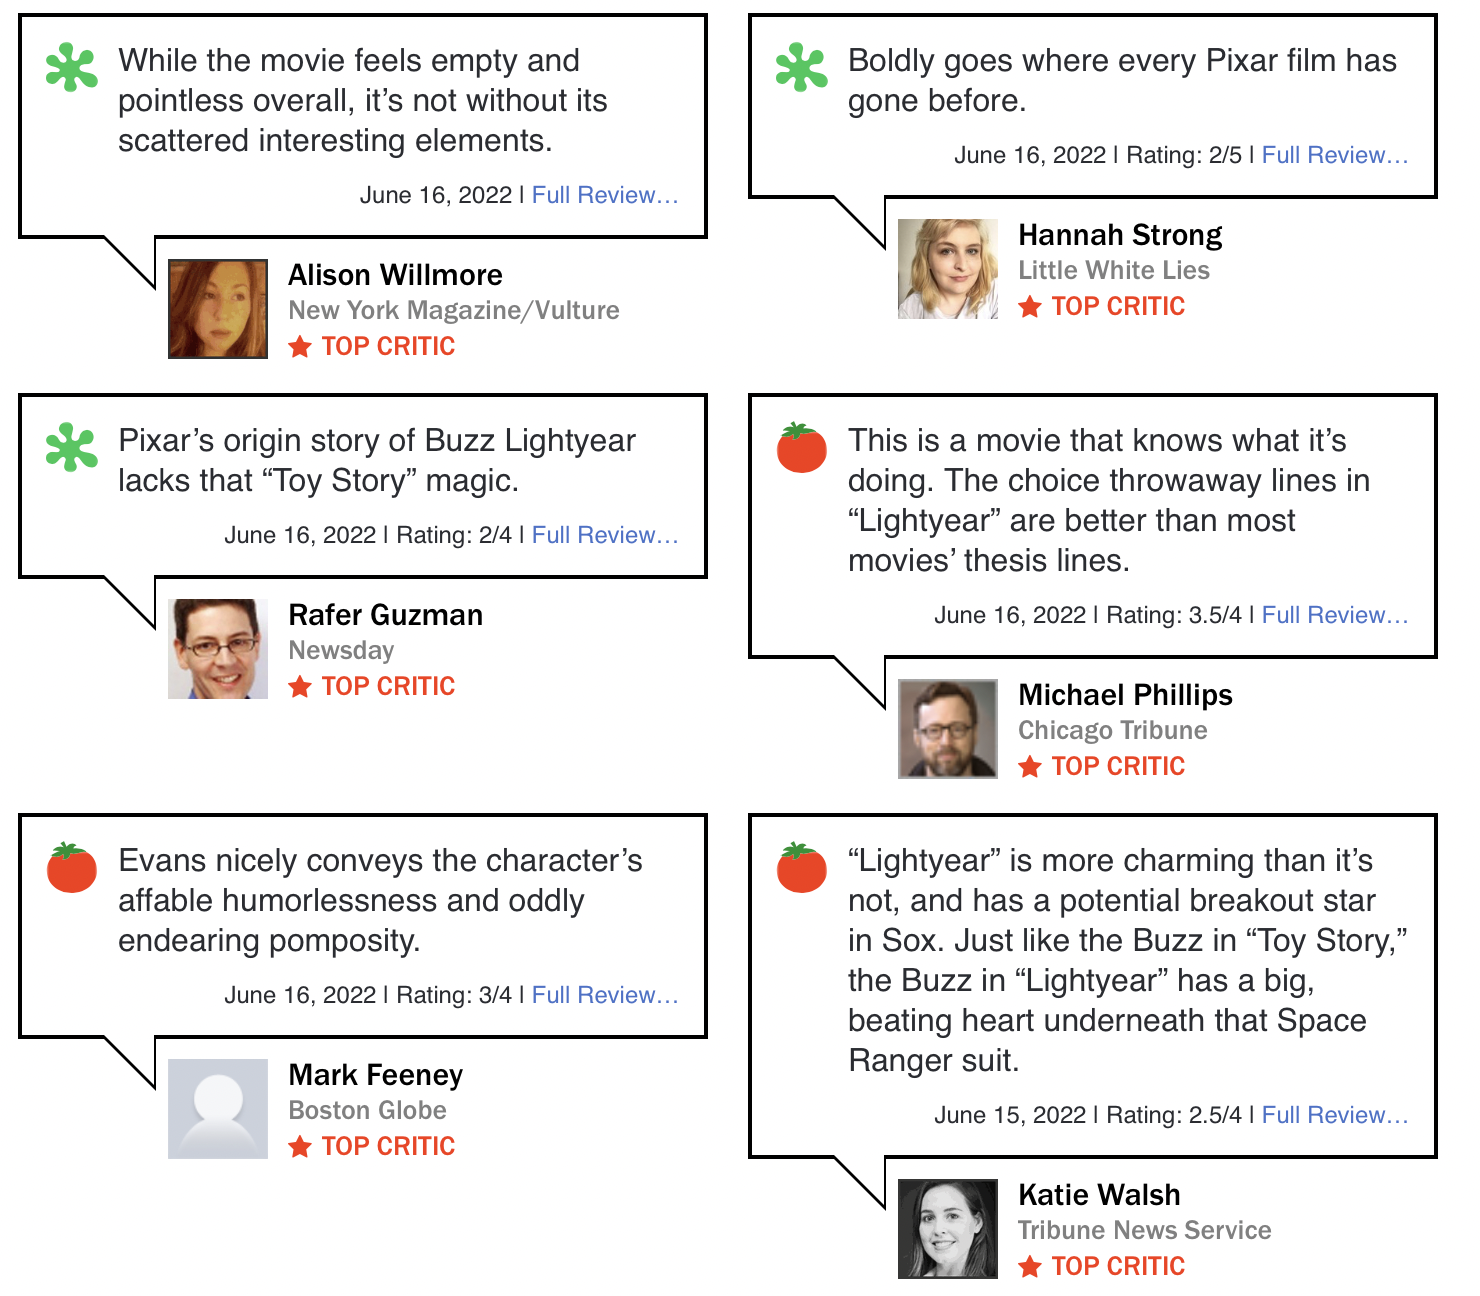
\includegraphics[scale=0.25]{img/rotten-tomatoes-comments.png}
    \caption{ Interfaz de comentarios de Rotten Tomatoes }
    \label{fig:rotten_tomatoes}
\end{figure}

Por su parte, \href{https://letterboxd.com}{Letterboxd} sí que se siente más como una red social centrada en las reseñas. Dándoles más importancia en el feed principal de la aplicación, en el que aparecen tanto las reseñas populares entre demás usuarios y las de los usuarios que tú sigues. También permite comentar las reseñas de los demás usuarios. Además, ofrece información sobre las distintas películas de la base de datos. De esta forma, Letterboxd se ofrece como una solución mucho más acertada a los problemas planteados en este proyecto.\\
\begin{figure}[H]
    \centering	
    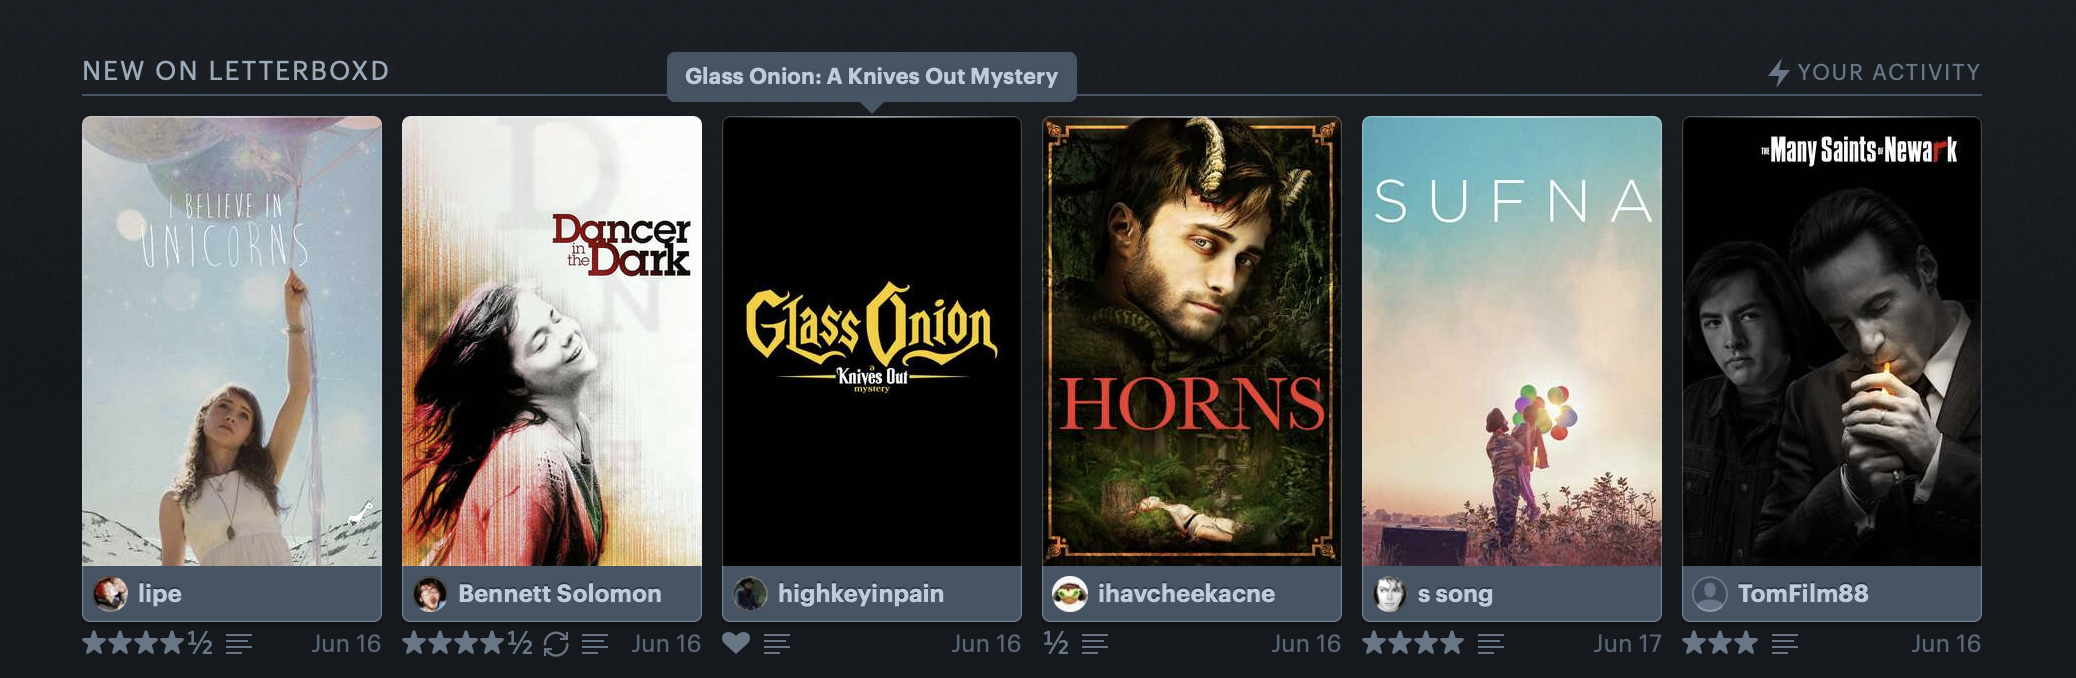
\includegraphics[scale=0.4]{img/letterboxd-feed.png}
    \caption{ Feed de la aplicación Letterboxd }
    \label{fig:letterboxd}
\end{figure}

Entonces, ¿por qué realizar una nueva aplicación? Los dos inconvenientes de Letterboxd son su interfaz algo desfasada y que solo permite realizar reseñas de películas, por lo que nuestros usuarios \textit{seriéfilos} son dejados de lado en esta aplicación.
